\documentclass[
	11pt, % Default font size
]{beamer}

\graphicspath{{Images/}{./}} % Path for included images

\usepackage{booktabs} % Improved table formatting
\usepackage{amsmath} % For better math formatting

%----------------------------------------------------------------------------------------
%	LAYOUT, COLOR, FONT, INNER AND OUTER THEME SELECTION
%----------------------------------------------------------------------------------------

\usetheme{Madrid} % Layout theme
\usecolortheme{dove} % Color theme
\usefonttheme{default} % Default sans-serif font
\useinnertheme{circles} % Inner theme for bullet points
\setbeamertemplate{footline}[page number] % Display page numbers
\setbeamertemplate{navigation symbols}{} % Remove navigation symbols

\usepackage{palatino} % Serif font for text
\usepackage[default]{opensans} % Open Sans for sans-serif text

%----------------------------------------------------------------------------------------
%	PRESENTATION INFORMATION
%----------------------------------------------------------------------------------------

\title[Deradicalize the Algorithm]{How to Deradicalize the Recommendation Algorithm: A Statistical Approach}
\subtitle{A Data-Driven Framework}
\author[Rodr\'iguez Caballero]{Jos\'e Manuel Rodr\'iguez Caballero}
\institute[ULaval]{Department of Mathematics and Statistics\\Faculty of Science and Engineering\\Universit\'e Laval}
\date[\today]{\today}

%----------------------------------------------------------------------------------------
%	START OF DOCUMENT
%----------------------------------------------------------------------------------------

\begin{document}

%----------------------------------------------------------------------------------------
%	TITLE SLIDE
%----------------------------------------------------------------------------------------

\begin{frame}
    \titlepage
\end{frame}

%----------------------------------------------------------------------------------------
%	INTRODUCTION
%----------------------------------------------------------------------------------------

\begin{frame}
	\frametitle{Overview}
	\tableofcontents
\end{frame}

\section{Motivation}
\begin{frame}
	\frametitle{Hebb's Rule}
    \begin{center}
	\emph{Neurons that fire together, wire together.}
    \end{center}
	\begin{figure}
		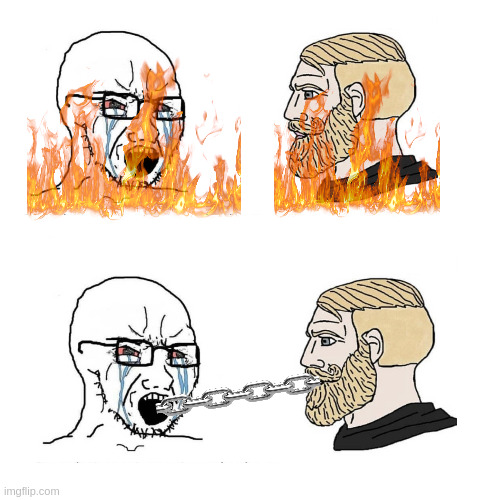
\includegraphics[width=0.4\linewidth]{947tkb.jpg}
		\caption{Hebb's Rule illustrated with memes.}
	\end{figure}
	\small{This behavior can lead to correlation between users' preferences over time, potentially spreading both neutral and extreme content through recommendation algorithms.}
\end{frame}

%----------------------------------------------------------------------------------------
%	RECOMMENDATION ALGORITHMS
%----------------------------------------------------------------------------------------

\section{Recommendation Algorithms}
\begin{frame}
    \frametitle{Recommendation Algorithms}
	According to NVIDIA\footnote{\url{https://www.nvidia.com/en-us/glossary/recommendation-system/}}: 
	\begin{quote}
A recommendation system (or recommender system) is a class of machine learning that uses data to help predict, narrow down, and find what people are looking for among an exponentially growing number of options.
	\end{quote}
    
\end{frame}

\section{Hebbian Algorithms}
\begin{frame}
    \frametitle{Hebbian Algorithms}
    A recommendation algorithm is termed \emph{Hebbian} if it satisfies:
    \begin{quote}
        \textbf{Property:} If two users (Alice and Bob) share many common products, recommendations for Alice will be influenced by Bob’s history, and vice versa.
    \end{quote}
    \vspace{0.2cm}
    \textbf{Potential Issue:} In this framework, users can unknowingly influence each other's recommendations, leading to unintended sociological consequences.
\end{frame}

\begin{frame}
    \frametitle{Example of Hebbian Algorithm}
    Consider the following simplified model of a Hebbian algorithm:
    \[
    P(\text{Recommend } x \text{ to Alice}) = \frac{\text{\# of times Bob consumed } x}{\text{\# of items Bob consumed}}.
    \]
    \vspace{0.3cm}
    \textbf{Comment:} This model assumes the influence between users is directly proportional to shared consumption, but real-world systems typically involve more complex patterns.
\end{frame}

%----------------------------------------------------------------------------------------
%	RADICALIZATION PROBLEM
%----------------------------------------------------------------------------------------

\section{Radicalization Pathway}
\begin{frame}
    \frametitle{Pathway to Radicalization}
    \textbf{Problem:} If Bob is radicalized and Alice shares many common interests, a Hebbian algorithm could unintentionally expose Alice to radical content.
    
    \begin{figure}
		
\includegraphics[width=0.5\linewidth]{947x9m.jpg}
		\caption{Radical content spreads via common user connections.}
	\end{figure}
\end{frame}

%----------------------------------------------------------------------------------------
%	PROPOSED SOLUTION
%----------------------------------------------------------------------------------------

\section{Proposed Solution}
\begin{frame}
    \frametitle{Proposed Solution: Statistical Intervention}
    \textbf{1. Identification of Radicalized Users:}
    \begin{itemize}
        \item Apply classification algorithms to detect users exhibiting extreme behavior patterns.
    \end{itemize}

    \textbf{2. Exclusion from Collaborative Filtering:}
    \begin{itemize}
        \item Ensure that consumption patterns from identified users are excluded from influencing other users' recommendations.
    \end{itemize}
    
    \textbf{3. Deradicalization Content:}
    \begin{itemize}
        \item Target radicalized users with curated content designed to counter extremist views.
    \end{itemize}
\end{frame}

%----------------------------------------------------------------------------------------
%	MEASURING SUCCESS
%----------------------------------------------------------------------------------------

\section{Measuring Success}
\begin{frame}
    \frametitle{Measuring Success: Statistical Approach}
    \textbf{Key Evaluation Metric: Reduction in Radicalized Recommendations}
    \vspace{0.2cm}
    
    \textbf{1. Pre-Implementation:}
    \begin{itemize}
        \item Sample users and record radicalized recommendations over a period (e.g., one month).
    \end{itemize}
    
    \textbf{2. Post-Implementation:}
    \begin{itemize}
        \item Measure radicalized recommendations after applying the exclusion method.
    \end{itemize}
    
    \textbf{3. Statistical Testing:}
    \begin{itemize}
        \item Conduct a \emph{paired t-test} to compare pre- and post-implementation recommendation counts.
        \item Estimate the effect size (e.g., Cohen's $d$) to quantify the impact of the intervention.
    \end{itemize}
\end{frame}

%----------------------------------------------------------------------------------------
%	END SLIDE
%----------------------------------------------------------------------------------------

\begin{frame}[plain] % The optional argument 'plain' hides the headline and footline
	\begin{center}
		{\Huge Thank You!}
	\end{center}
\end{frame}

%----------------------------------------------------------------------------------------
\end{document}
